% Jacob Neumann

% DOCUMENT CLASS AND PACKAGE USE
    \documentclass[aspectratio=169, handout]{beamer}

    % Establish the colorlambda boolean, to control whether the lambda is solid color (true), or the same as the picture (false)
    \newif\ifcolorlambda
    \colorlambdafalse % DEFAULT: false

    % Use auxcolor for syntax highlighting
    \newif\ifuseaux
    \useauxfalse % DEFAULT: false

    % Color settings
    \useauxtrue

    \newcommand{\auxColor}{c9a500}     % the color of note boxes and stuff
    \newcommand{\presentColor}{BB5D07} % the primary color of the slide borders
    \newcommand{\bgColor}{fff1e8}      % the color of the background of the slide
    \newcommand{\darkBg}{8b98ad}
    \newcommand{\lambdaColor}{\auxColor}

    \colorlambdatrue

    \usepackage{comment} % comment blocks
    \usepackage{soul} % strikethrough
    \usepackage{listings} % code
    \usepackage{makecell}

    \setbeamertemplate{itemize items}[circle]
    % \setbeameroption{show notes on second screen=right}

    \usepackage{lectureSlides}
    %%%%%%%%%%%%%%%%%%%%%%%%%%%%%%%%%%%%%%%%%| <----- Don't make the title any longer than this
    \title{Modules I: Structures and Signatures} % TODO
    \subtitle{Structuring software} % TODO
    \date{06 July 2023} % TODO
    \author{Brandon Wu} % TODO

    \graphicspath{ {./img/} }
    % DONT FORGET TO PUT [fragile] on frames with codeblocks, specs, etc.
        %\begin{frame}[fragile]
        %\begin{codeblock}
        %fun fact 0 = 1
        %  | fact n = n * fact(n-1)
        %\end{codeblock}
        %\end{frame}

    % INCLUDING codefile:
        % 1. In some file under code/NN (where NN is the lecture id num), include:
    %       (* FRAGMENT KK *)
    %           <CONTENT>
    %       (* END KK *)

    %    Remember to not put anything on the same line as the FRAGMENT or END comment, as that won't be included. KK here is some (not-zero-padded) integer. Note that you MUST have fragments 0,1,...,KK-1 defined in this manner in order for fragment KK to be properly extracted.
        %  2. On the slide where you want code fragment K
                % \smlFrag[color]{KK}
        %     where 'color' is some color string (defaults to 'white'. Don't use presentColor.
    %  3. If you want to offset the line numbers (e.g. have them start at line 5 instead of 1), use
                % \smlFragOffset[color]{KK}{5}

    \usetikzlibrary{calc}
    \tikzset{
      between/.style args={#1 and #2}{
        at = ($(#1)!0.5!(#2)$)
      }
    }

\begin{document}

% Make it so ./mkWeb works correctly
\ifweb
    \renewcommand{\pause}{}
\fi

\setbeamertemplate{itemize items}[circle]

% SOLID COLOR TITLE (see SETTINGS.sty)
{
\begin{frame}[plain]
    \colorlambdatrue
    \titlepage
\end{frame}
}

\menti{4624 1952}

\begin{frame}[fragile]
  \frametitle{Lesson Plan}

  \tableofcontents
\end{frame}

\sectionSlide{1}{Structures and Namespaces}

\begin{frame}[fragile]
  \frametitle{Organizing Software}

  So far we have explored the core SML language features that let us write
  interesting functions.

  \pause
  \vspace{\fill}

  We've seen functions and datatypes, exceptions and variables, and many
  applications thereof. These are essential for the purpose of solving interesting
  problems, but what about problems that are not strictly computational?

  \pause
  \vspace{\fill}

  Code is not just meant to be written, it is meant to be used,
  documented, and organized. We are interested in the problem of organizing software.
\end{frame}

\begin{frame}[fragile]
  \frametitle{Namespaces}

  One particular idea for organizing software is the idea of \term{namespaces}.

  \pause
  \vspace{\fill}

  \defBox{}{A \term{namespace} is a particular group of defined elements which
  live separately from others. In a programming language, there will usually be
  ways of referring to different namespaces, to separate out used names from each
  other.}

  \pause
  \vspace{\fill}

  For instance, we exhibit this with the syntax that we have used so far, with
  names such as \code{List.length} and \code{Int.compare}. The \code{compare}
  function lives in the namespace associated to \code{Int}, and the \code{length}
  function lives in the namespace associated to \code{List}.

  \pause
  \vspace{\fill}

  \noteBox{}{This means there could be definitions of the same name in different
  namespaces! We could have separate \code{List.compare} and \code{Int.compare}
  functions.}
\end{frame}

\begin{frame}[fragile]
  \frametitle{Structures}

  It turns out that \code{List} and \code{Int} are just examples of what SML
  calls \term{modules}, or \term{structures}.

  \pause
  \vspace{\fill}

  \defBox{}{A \term{module} or \term{structure} is a grouping of declarations
  underneath a particular name.}

  \pause
  \vspace{\fill}

  For instance, we could write the following syntax:
  \begin{codeblock}
    structure Foo =
      struct
        datatype t = Bar of int
        val x = Bar 5
        exception E of t
      end
  \end{codeblock}

  such that the names \code{t}, \code{Bar}, \code{x}, and \code{E} are entirely
  local to the structure \code{Foo}.

\end{frame}

\begin{frame}[fragile]
  \frametitle{Separation of Concerns}

  This means that outside the structure, we could write:

  \begin{codeblock}
    val y = Foo.Bar 1
    val z = raise Foo.E y
  \end{codeblock}
  to access the inner contents.

  \pause
  \vspace{\fill}

  This is helpful for when we're working with many definitions, and we want to
  group them distinctly! For instance, we might be interested in functions specific
  to a particular part of our codebase. With modules, we can group domain-specific logic under the
  module for that specific application.

  \pause
  \vspace{\fill}

  \noteBox{}{Because modules can contain exceptions and types, and their
  components can be referred to by name, they are more powerful than just simple
  tuples, which can only contain values organized by position!\footnote{
    Technically, SML has a notion of \term{records}, which are
    tuples with fields organized by name. But records also can only contain
    values, and not things like types.
  }}
\end{frame}

\begin{frame}[fragile]
  \frametitle{A Collection of Definitions}

  How does this differ from just organizing the contents of modules into
  their own files? For one, files do not promote their own personal
  namespacing in the same way as modules. If we have two files, with contents:

  \begin{codeblock}
    val x = 2
  \end{codeblock}

  \begin{codeblock}
    val y = 3
  \end{codeblock}

  then loading both of these SML files will result in an environment containing
  both \code{x} and \code{y}. We want to be able to separate out unrelated parts
  by more than just the file they are located in.

  \pause
  \vspace{\fill}

  But, modules share the same drawbacks as files in other senses. Both are just
  collections of definitions, at the end of the day. Consider the problem of
  the \code{msort} function.
\end{frame}

\begin{frame}[fragile]
  \frametitle{An Example File}

  {\tiny
  \begin{codeblock}
    fun split [] = ([], [])
      | split [x] = ([x], [])
      | split (x::y::xs) =
          let
            val (A, B) = split xs
          in
            (x::A, y::B)
          end

    fun merge ([], R) = R
      | merge (L, []) = L
      | merge (x::xs, y::ys) =
          case Int.compare (x, y) of
            LESS => x :: merge (xs, y::ys)
          | _ => y :: merge (x::xs, ys)

    fun msort [] = []
      | msort [x] = [x]
      | msort L =
          let
            val (A, B) = split L
          in
            merge (msort A, msort B)
          end
  \end{codeblock}
  }

  \pause
  \vspace{\fill}

  Here's an example of a potential SML file, call it \code{msort.sml}.
\end{frame}

\begin{frame}[fragile]
  \frametitle{Namespace Clutter}

  The pitfalls of packaging code as just a collection of definitions is
  that there's no way to be clear about which parts are important!

  \pause
  \vspace{\fill}

  The definition of \code{msort} relies on two helper functions, \code{merge}
  and \code{split}. We cannot avoid writing these functions, but because they
  are written at the top-level, loading this SML file will also load those
  functions into the namespace automatically.

  \pause
  \vspace{\fill}

  This causes \term{namespace clutter}, because now we have introduced two
  definitions for \code{merge} and \code{split}, when we only wanted them
  for the purpose of writing \code{msort}!
\end{frame}

\begin{frame}[fragile]
  \frametitle{A Local Approach}

  One way to get around this is with something called a \term{local definition}.

  \pause
  \vspace{\fill}

  This looks like:

  \begin{codeblock}
    local
      fun split L = (* ... *)
      fun merge (L1, L2) = (* ... *)
    in
      fun msort [] = []
        | msort [x] = [x]
        | msort L = (* ... *)
    end
  \end{codeblock}

  \pause
  \vspace{\fill}

  This form makes it more clear where the dependencies are. But it's also a burden
  on the writer of the code! We'd like a solution which ideally doesn't burden
  the source code.
\end{frame}

\begin{frame}[fragile]
  \frametitle{What's in a File?}

  Additionally, we want to make it very clear to a user of a library, what the
  contents of the library are, and what it approximately does. How can we somehow
  convey the contents of a collection of code, without necessarily needing to alter
  the source significantly?

  \pause
  \vspace{\fill}

  We could just write this at the top of the file, for instance:

  \begin{codeblock}
    (* This file contains `msort : int list -> int list' *)

    (* IGNORE *)
    fun split L = (* ... *)
    fun merge (L1, L2) = (* ... *)
    fun msort L = (* ... *)
  \end{codeblock}

  \pause
  But now, what happens if we refactor our code?
\end{frame}

\begin{frame}[fragile]
  \frametitle{What's in a File?}

  \begin{codeblock}
    (* This file contains `msort : int list -> int list' *)

    (* IGNORE *)
    fun split L = (* ... *)
    fun merge `cmp` (L1, L2) = (* ... *)
    fun msort `cmp` L = (* ... *)
  \end{codeblock}

  Suppose that we change our implementation of \code{msort}, to one
  which is now \code{msort : ('a * 'a -> order) -> 'a list -> 'a list}.

  \pause
  \vspace{\fill}

  Well, now we have to go and change our documentation! Our comment
  isn't actually checked for accuracy, so it might be the case that it
  gets outdated. We can't necessarily trust documentation, because it's
  not verified by anything.

  Can we do better?
\end{frame}

\begin{frame}[fragile]
  \frametitle{An Interface}

  \customBox{Idea}{\, What if we had an interface for our file that was
  checked by the compiler?}

  \pause
  \vspace{\fill}

  What kind of information are we interested in having present in this interface?

  \pause
  \vspace{\fill}

  We will check for:
  \pause
  \begin{itemize}
    \item the presence of certain declarations \pause
    \item the type of value bindings within the file
  \end{itemize}

  \pause
  \vspace{\fill}

  This is the idea of a \term{signature}.
\end{frame}

\sectionSlide{2}{Signatures and Interfaces}

\begin{frame}[fragile]
  \frametitle{Signatures}

  \defBox{}{A \term{signature} is an SML construct, consisting of a collection
  of \term{specifications} for things such as types, values, and exceptions.}

  \pause
  \vspace{\fill}

  Here is an example of a signature we could have for a module containing our
  \code{msort} code, instead of putting it into a separate file \code{msort.sml}:

  \begin{codeblock}
    signature MSORT =
      sig
        val msort : ('a * 'a -> order) -> 'a list -> 'a list
      end
  \end{codeblock}

  \vspace{\fill}

  By convention, we usually put the name of a signature in all-caps.

  \pause
  \vspace{\fill}

  This is the signature of a module which publicly contains just a single value,
  which is a function \code{msort} of type \code{('a * 'a -> order) -> 'a list -> 'a list}.
\end{frame}

\begin{frame}[fragile]
  \frametitle{A Module for \code{msort}}

  Suppose we wanted to define our new shiny \code{Msort} module. We might write:

  \pause
  \begin{codeblock}
    structure Msort =
      struct
        fun split L = (* ... *)
        fun merge cmp (L1, L2) = (* ... *)
        fun msort cmp L = (* ... *)
      end
  \end{codeblock}

  \pause
  \vspace{\fill}

  Now, we can access our \code{msort} function via \code{Msort.msort}.

  \pause
  \vspace{\fill}

  But, we haven't yet looped in our \code{MSORT} signature! This means that
  as currently written, we can still write \code{Msort.split} and \code{Msort.merge}.
  We also don't have any check that \code{msort} is truly of type
  \code{('a * 'a -> order) -> 'a list -> 'a list}.
\end{frame}

\begin{frame}[fragile]
  \frametitle{Ascription}

  \defBox{}{The act of specifying that a module should implement a given
  signature is called \term{ascription}.}

  \pause
  \vspace{\fill}

  To ensure that our \code{Msort} module has to be compatible with the
  \code{MSORT} signature, we have to perform \term{ascription}. We write it
  like this:

  \begin{codeblock}
    structure Msort `: MSORT` =
      struct
        fun split L = (* ... *)
        fun merge cmp (L1, L2) = (* ... *)
        fun msort cmp L = (* ... *)
      end
  \end{codeblock}

  \pause
  \vspace{\fill}

  This means that, after this ascription, the \textit{only declarations} that
  are visible within \code{Msort} from a user are the declarations contained
  within the \code{MSORT} signature!
\end{frame}

\begin{frame}[fragile]
  \frametitle{Ascription and Typechecking}

  \tgs

  This means that we cannot use \code{Msort.split} or \code{Msort.merge},
  because we're restricted to knowledge of the interface.

  \pause
  \vspace{\fill}

  The other great advantage of ascription is that it only succeeds if
  all of the declarations that are present in the signature are present in
  the structure, \textit{and} the declarations in the structure must have
  consistent types with those in the signature.

  \pause
  \vspace{\fill}

  So if we implemented \code{msort} with any type other than
  \code{('a * 'a -> order) -> 'a list -> 'a list}, the program would
  fail to compile. This means that our interfaces are not just well-specified,
  but significantly stronger than comments. They are guaranteed to be safe.
\end{frame}

\sectionSlide{3}{Abstraction}

\begin{frame}[fragile]
  \frametitle{Abstraction Boundaries}

  One of the greatest wins in computer science is the idea of \term{abstraction}.

  \pause
  \vspace{\fill}

  This means, essentially, deliberately forming higher-level models of things which
  ignore irrelevant details. This helps us a lot in understanding things with our
  human brains. For instance, we choose to think about evaluation of expressions,
  rather than flipping of bits in computer hardware.

  \pause
  \vspace{\fill}

  At the software level, abstraction abounds as well. We want to choose to
  ignore the parts of implementations that do not matter to us. This is the
  entire point of specifications.

  \pause
  \vspace{\fill}

  Signatures and structures offer us a way to enforce this idea of abstraction.
\end{frame}

\begin{frame}[fragile]
  \frametitle{An Abstract Sort}

  The way that we defined \code{MSORT} and \code{Msort} earlier are actually
  in violation of this idea of abstraction!

  \pause
  \vspace{\fill}

  Consider the signature \code{MSORT}:

  \begin{codeblock}
    signature MSORT =
      sig
        val msort : ('a * 'a -> order) -> 'a list -> 'a list
      end
  \end{codeblock}

  \pause
  \vspace{\fill}

  Why is it important to me, as a user of this sorting library, that it
  is implemented as a merge sort? The reason why I am using it is that I
  want a sorted list -- but the concrete implementation details
  \textbf{do not matter} to me.\footnote{The astute reader might raise complaints about how it
  may be important to know the run-time complexity of the sorting function.
  Merge sort isn't the only $O(n \log n)$ sorting algorithm out there, though,
  and generally when using a library, you should be able to trust that the
  authors implemented it in a vaguely efficient way.}
\end{frame}

\begin{frame}[fragile]
  \frametitle{Abstracting Implementation}

  Here's a better signature:

  \begin{codeblock}
    signature `SORT` =
      sig
        val `sort` : ('a * 'a -> order) -> 'a list -> 'a list
      end
  \end{codeblock}

  \pause
  \vspace{\fill}

  We changed very little, but the idea is that we want to remove as many irrelevant
  details as possible from the users of the library! They want a sort, and they
  get a sort. The name is suggestive enough.
\end{frame}

\begin{frame}[fragile]
  \frametitle{Alternate Implementation}

  Another reason for doing this, is that we might define multiple sorting libraries,
  and we want them to ascribe to a common signature! So now, we can also define a
  \code{InsertionSort} module:

  \pause
  \vspace{\fill}

  \begin{codeblock}
    structure InsertionSort : SORT =
      struct
        fun sort cmp L = (* ... *)
      end
  \end{codeblock}
\end{frame}

\quizBreak{MODULARITY}

\sectionSlide{4}{Information Hiding}

\begin{frame}[fragile]
  \frametitle{Types in Structures}

  Recall that structures can also contain types. Consider a signature which
  describes a library for sets of integers.

  \pause
  \vspace{\fill}

  \begin{codeblock}
    signature INTSET =
      sig
        type t

        val empty : t
        val insert : int -> t -> t
        val remove : int -> t -> t
        val mem : int -> t -> bool
      end
  \end{codeblock}

  \pause
  \vspace{\fill}

  We call the type \code{t} in this signature \term{abstract}, because it
  is left unspecified! Structures which implement this signature (or \term{ascribe}
  to it) can choose whatever representation they want.
\end{frame}

\begin{frame}[fragile]
  \frametitle{Types in Structures}

  Consider a structure which implements \code{INTSET} with lists.

  \pause
  \small
  \begin{codeblock}
    structure IntSet : INTSET =
      struct
        type t = int list

        val empty = []
        fun insert v [] = [v]
          | insert v (x::xs) =
              if v = x then x::xs
              else (x :: insert v xs)
        fun remove v [] = []
          | remove v (x::xs) =
              if v = x then xs
              else (x :: remove v xs)
        fun mem v [] = false
          | mem v (x::xs) = v = x orelse mem v xs
      end
  \end{codeblock}
\end{frame}

\begin{frame}[fragile]
  \frametitle{Opening Up}

  \begin{center}
    \includegraphics[scale=0.35]{open}
  \end{center}

  \noteBox{}{The \code{open} keyword allows you to open all the things in a
  module into the enclosing scope.}

  \pause
  \vspace{\fill}

  The important thing is the line \code{type t = int list}.
\end{frame}

\begin{frame}[fragile]
  \frametitle{Transparent Ascription}

  The type of ascription we showed you earlier is called \term{transparent ascription}.

  \pause
  \vspace{\fill}

  The key thing that it does is that, even though the type of \code{t} in the
  signature \code{INTSET} is unspecified, transparent ascription makes it so that
  the type of \code{IntSet.t} is publicly known to be \code{int list}.

  \pause
  \vspace{\fill}

  This is \textbf{really bad}.
\end{frame}

\begin{frame}[fragile]
  \frametitle{I'm Gonna Wreck It}

  Because \code{IntSet.t} is the same as \code{int list}, it is OK to write
  the following:

  \pause
  \begin{codeblock}
    val set : IntSet.t = [1, 1, 1, 1]

    val set_without_1_i_promise = IntSet.remove 1 set

    val _ =
      if IntSet.mem 1 set_without_1_i_promise then
        destroy_universe ()
      else
        dont ()
  \end{codeblock}

  \pause
  \vspace{\fill}

  This code destroys the universe.\footnote{Sometimes that happens.}
\end{frame}

\begin{frame}[fragile]
  \frametitle{Invariant Violation}

  What happened here? We violated an invariant.

  \pause
  \vspace{\fill}

  The \code{IntSet} library was carefully constructed so that by using
  \code{empty}, \code{insert}, and \code{remove}, every set would act like
  a set -- in particular, \code{mem x (remove x S)} $\eeq$ \code{false}. Every
  set should have precisely at most one entry for each integer.

  \pause
  \vspace{\fill}

  When outside users of the library know \textit{how it's implemented}, they
  can violate this invariant! This means if there was code somewhere which
  relied on receiving an \code{IntSet.t}, we could mess them up.

  \pause
  \vspace{\fill}

  So how do we prevent this?
\end{frame}

\begin{frame}[fragile]
  \frametitle{Opaque Ascription}

  The converse to transparent ascription is called \term{opaque ascription}.

  \pause
  \vspace{\fill}

  \defBox{}{\term{Opaque ascription} is transparent ascription, but any
  abstract types in the signature are unknown to users of the structure.}

  \pause
  \begin{codeblock}
    structure IntSetOpaque `:>` INTSET =
      struct
        type t = int list

        val empty = []
        (* ... *)
        fun mem v [] = false
          | mem v (x::xs) = v = x orelse mem v xs
      end
  \end{codeblock}

  Here's how we write it.
\end{frame}

\begin{frame}[fragile]
  \frametitle{Invariants, Invincible}

  \tgs

  In the resulting structure \code{IntSetOpaque}, users of the module have
  no idea that the type \code{IntSetOpaque.t} is \code{int list}, and the compiler will
  enforce that. The compiler will fail to recognize that \code{IntSetOpaque.t}
  is the same as \code{int list}. We have \textbf{hidden} the fact that the
  \code{IntSetOpaque} library is implemented with lists.

  \pause
  \vspace{\fill}

  This means that now it is \textit{impossible} to obtain a value of type
  \code{IntSetOpaque.t} without going through \code{IntSetOpaque.empty},
  \code{IntSetOpaque.remove}, or \code{IntSetOpaque.insert}. This means that
  now it is \textbf{provably impossible} to ever break our set invariant.

  \pause
  \vspace{\fill}

  That's pretty neat.
\end{frame}

\begin{frame}[fragile]
  \frametitle{Using Opaque Structures}

  \begin{center}
    \includegraphics[scale=0.35]{open2}
  \end{center}
\end{frame}

\begin{frame}[fragile]
  \frametitle{Using Opaque Structures}

  Now, we cannot see what the type \code{t} is at all, and it will
  not type-check if we try to declare a list to be of type
  \code{IntSetOpaque.t}.

  \pause
  \vspace{\fill}

  \begin{center}
    \includegraphics[scale=0.45]{opaque_cast}
  \end{center}
\end{frame}


\begin{frame}[fragile]
  \frametitle{On Users and Maintainers}

  Again, this might seem strange. We just implemented \code{IntSetOpaque} as an
  \code{int list} like five minutes ago, what do you mean we don't know it's an
  \code{int list}?

  \pause
  \vspace{\fill}

  The idea is that \textbf{signatures are for the user}, and \textbf{structures
  are for the maintainer}. The user of a library should only have to know things
  which are in the interface, and the implementation details are left to the
  maintainer, in the structure.

  \pause
  \vspace{\fill}

  Being a programmer is a tenuous dance, because you're both. You implement libraries
  that you end up using, meaning you are both consumer and producer. Why is this
  important?
\end{frame}

\begin{frame}[fragile]
  \frametitle{On Users and Maintainers}

  There are several advantages to being able to close your eyes and think like a
  user, rather than a maintainer:

  \pause
  \begin{itemize}
    \item \textbf{it lightens your conceptual load}. Instead of thinking about the implementation
    of \code{insert}, \code{remove}, and co, you can think intuitively about what
    a set is. \pause
    \item \textbf{it prevents you from breaking your own invariants}. If you set your invariants
    ahead of time, and design your API so you can never break it through the interface,
    then being unable to access the representation from outside the library prevents
    you from mangling your invariants later. \pause
    \item \textbf{it helps you maintain your code}. If you later decide to refactor your code
    to use a different representation, such as a \code{int tree}, you don't need to
    touch any of the code outside of the module, so long as you adhere to the
    original interface.
  \end{itemize}

  \pause
  \vspace{\fill}

  SML's ability to \textit{enforce} that you don't break this abstraction layer
  is one of the most powerful benefits that it provides.
\end{frame}

\sectionSlide{5}{Representation Independence}

\begin{frame}[fragile]
  \frametitle{Thinking Conceptually}

  So far in this course, we've trained our brains to be like mini-SML interpreters,
  such that we generally understand the stepping that SML programs will do, when we
  feed them into SML/NJ.

  \pause
  \vspace{\fill}

  Something that has been mentioned several times in the past, however, is that
  this is ultimately inefficient! We can't think about stepping arbitrarily complex
  expressions in our head, because it will become too much mental load.

  \pause
  \vspace{\fill}

  A more powerful tool we've relied on is using \textit{invariants}, and in particular
  \code{ENSURES} postconditions, to reason about why recursive functions should be
  correct.

  \pause
  \vspace{\fill}

  With representation independence, we can do even better. We can rely on \textit{pictures}
  to reason about our code.
\end{frame}

\begin{frame}[fragile]
  \frametitle{Thinking Conceptually}

  For instance, take the following code:

  \pause
  \vspace{\fill}

  {\small
  \begin{codeblock}
    IntSet.insert 3 (IntSet.insert 2 (IntSet.insert 1 IntSet.empty))
  \end{codeblock}
  }

  \pause
  \vspace{\fill}

  Which is easier to think about -- this:

  \begin{center}
    {\color{blue} \href{https://asciinema.org/a/x3HwtfZyK6TYkDQ9eA1NztuVR}{mulligan trace}
    }
  \end{center}

  \pause
  or this?

  \begin{center}
    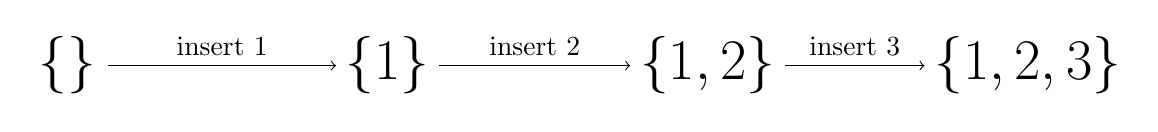
\begin{tikzpicture}
      [set/.style={minimum width=0.4in, node distance=1.6in},
      ]
      \node[set] (N1) {\huge $\{\}$};
      \node[set, right of=N1] (N2) {\huge $\{1\}$};
      \node[set, right of=N2] (N3) {\huge $\{1, 2\}$};
      \node[set, right of=N3] (N4) {\huge $\{1, 2, 3\}$};

      \draw[->] (N1) to node[above]{insert $1$} (N2);
      \draw[->] (N2) to node[above]{insert $2$} (N3);
      \draw[->] (N3) to node[above]{insert $3$} (N4);
    \end{tikzpicture}
  \end{center}
\end{frame}

\begin{frame}[fragile]
  \frametitle{Thinking Conceptually}

  Due to opacity disallowing visibility into what the code is \textit{really}
  doing, it ends up not mattering how the structure is actually implemented,
  so long as it \textit{behaves} the way that it should.

  \pause
  \vspace{\fill}

  This is the ultimate form of the duck test -- if it walks like a duck,
  swims like a duck, and quacks like a duck, then it's probably a duck. In this
  case, if it behaves like a set, you can think of it like a set.

  \pause
  \vspace{\fill}

  Now, instead of thinking of the code stepping in great detail, we just
  think of the picture in our head, of a set.
\end{frame}

\begin{frame}[fragile]
  \frametitle{Thinking Conceptually}

  This will lead to a related concept called \term{representation independence}.

  \pause
  \vspace{\fill}

  \defBox{}{\term{Representation independence} is the phenomena where use of a
  library is independent of how it is represented. Ideally, any library involving
  an abstract type should be representationally independent.
  }

  \pause
  \vspace{\fill}

  For instance, let's think of the difference between the following two
  code fragments:

  \begin{codeblock}
    IntSet.insert 2 (IntSet.insert 1 IntSet.empty)
  \end{codeblock}

  \begin{codeblock}
    IntSet.insert 1 (IntSet.insert 2 IntSet.empty)
  \end{codeblock}
\end{frame}

\begin{frame}[fragile]
  \frametitle{Sets, Transparently}

  In terms of the concrete behavior of the function, we can see the actual
  value used to represent both, via using \code{IntSet} transparently:

  \begin{center}
    \includegraphics[scale=0.45]{rep}
  \end{center}

  We see that the actual value we obtain in either case, when we expose the
  inner representation, is \code{[1, 2]} and \code{[2, 1]}.

  \pause
  \vspace{\fill}

  Obviously, at this point in the course we recognize that those are different
  values. What gives? Isn't that an issue, since they are supposed to represent
  the same set?

  \pause
  \vspace{\fill}

  The answer is \textit{no}, and it's precisely because of this representationally
  independent thinking. Instead of thinking of values, we can group the values of
  the implementation into \textbf{representationally equivalent} classes, such that
  no two values in the same equivalence class can be distinguished.
\end{frame}

\begin{frame}[fragile]
  \frametitle{Representational Equivalence Classes}

  The picture might look like this:

  \begin{center}
    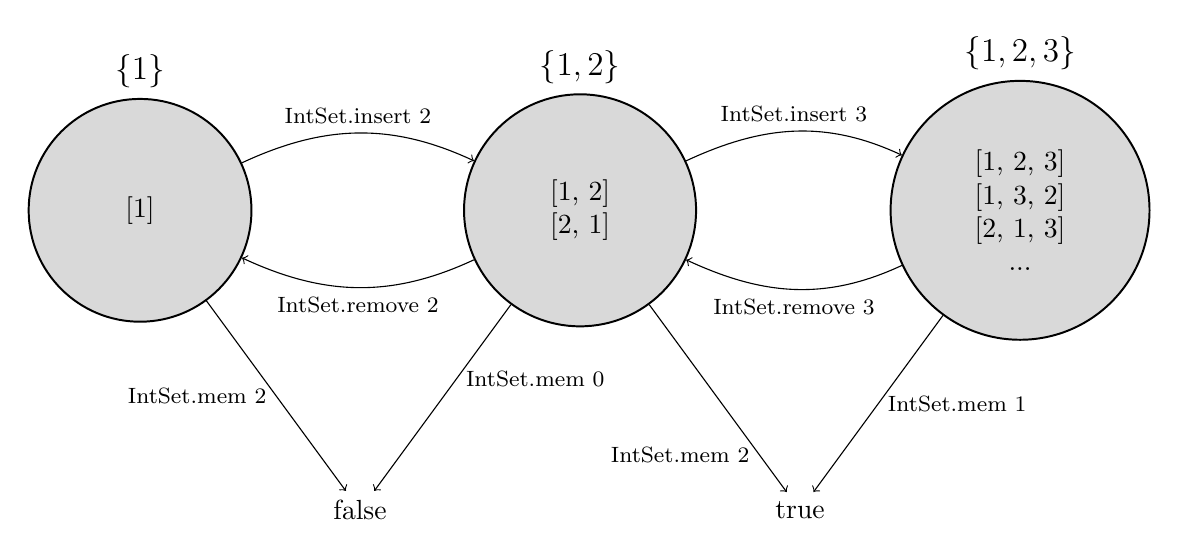
\begin{tikzpicture}
      [class/.style={align=center, text width=1in, draw=black, circle, fill=gray!30!white, line width=0.25mm},
      ]

      \node[label={\large $\{1\}$}, class] (N1) {\code{[1]}};
      \node[label={\large $\{1, 2\}$}, class, right of=N1, node distance=2.2in] (N2) {
        \code{[1, 2]} \\ \code{[2, 1]}
      };
      \node[label={\large $\{1, 2, 3\}$}, class, right of=N2, node distance=2.2in] (N3) {
        \code{[1, 2, 3]} \\
        \code{[1, 3, 2]} \\
        \code{[2, 1, 3]} \\
        ...
      };

      \node[between=N1 and N2, yshift=-1.5in] (F) {\code{false}};
      \node[between=N2 and N3, yshift=-1.5in] (T) {\code{true}};

      \draw[->] (N1) to [out=25, in=155] node[above]{\footnotesize \code{IntSet.insert 2}} (N2);
      \draw[->] (N2) to [out=25, in=155] node[above]{\footnotesize \code{IntSet.insert 3}} (N3);
      \draw[<-] (N1) to [out=-25, in=-155] node[below]{\footnotesize \code{IntSet.remove 2}} (N2);
      \draw[<-] (N2) to [out=-25, in=-155] node[below]{\footnotesize \code{IntSet.remove 3}} (N3);

      \draw[->] (N1) to node[left]{\footnotesize \code{IntSet.mem 2}} (F);
      \draw[->] (N2) to node[right, pos=0.4]{\footnotesize \code{IntSet.mem 0}} (F);

      \draw[->] (N2) to node[left, pos=0.8]{\footnotesize \code{IntSet.mem 2}} (T);
      \draw[->] (N3) to node[right]{\footnotesize \code{IntSet.mem 1}} (T);
    \end{tikzpicture}
  \end{center}
\end{frame}

\begin{frame}[fragile]
  \frametitle{Representational Equivalence Classes}

  \ptmt

  The previous image had many\footnote{In fact, infinitely many.} nodes and edges missing from it,
  but the basic idea is that the circles denote the representational equivalence
  classes for values which \textit{cannot be distinguished}, from outside
  the structure. They all denote the same basic mathematical set, which labels
  the circle at the top.

  \pause
  \vspace{\fill}

  This means that you can transform values within the classes into other classes
  via edges that correspond to functions like \code{IntSet.insert} and
  \code{IntSet.remove}, and no matter what the actual precise value is, it
  will still respect the equivalence classes and their arrows.

  \pause
  \vspace{\fill}

  In other words, you can define a \term{relation} on values, showing that
  they must always produce equivalently related values, from the same
  operations.
\end{frame}

\begin{frame}[fragile]
  \frametitle{Representation Independence for Trees}

  This is a generalizable idea, however! This kind of diagram isn't
  specific to lists, it might apply to any structure which chooses to
  implement \code{INTSET}, and does it in a faithful way. For instance,
  suppose we had implemented \code{IntSet} using trees.

  \pause
  \vspace{\fill}

  So now we might be able to draw a different picture, of what the same
  diagram looks like if we had implemented \code{IntSet} with trees. Note
  that for brevity, \code{Node} has been shortened to \code{N}, and
  \code{Empty} to \code{E}:
\end{frame}

\begin{frame}[fragile]
  \frametitle{Representational Equivalence Classes (Trees)}

  \begin{center}
    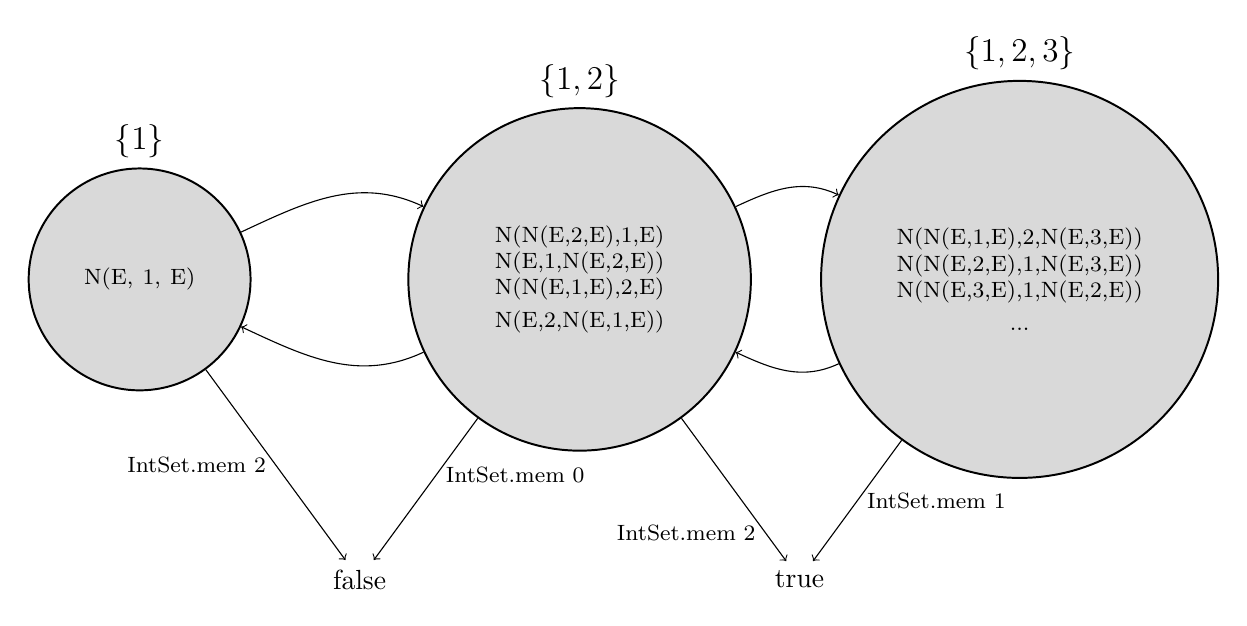
\begin{tikzpicture}
      [class/.style={align=center, text width=1.5in, draw=black, circle, fill=gray!30!white, line width=0.25mm},
      ]

      \node[label={\large $\{1\}$}, class, text width=1in] (N1) {\footnotesize \code{N(E, 1, E)}};
      \node[label={\large $\{1, 2\}$}, class, right of=N1, node distance=2.2in, text width=1.5in] (N2) {
        \footnotesize
        \code{N(N(E,2,E),1,E)} \\
        \code{N(E,1,N(E,2,E))} \\
        \code{N(N(E,1,E),2,E)} \\
        \code{N(E,2,N(E,1,E))}
      };
      \node[label={\large $\{1, 2, 3\}$}, class, right of=N2, node distance=2.2in, text width=1.8in] (N3) {
        \footnotesize
        \code{N(N(E,1,E),2,N(E,3,E))} \\
        \code{N(N(E,2,E),1,N(E,3,E))} \\
        \code{N(N(E,3,E),1,N(E,2,E))} \\
        ...
      };

      \node[between=N1 and N2, yshift=-1.5in] (F) {\code{false}};
      \node[between=N2 and N3, yshift=-1.5in] (T) {\code{true}};

      \draw[->] (N1) to [out=25, in=155] (N2);
      \draw[->] (N2) to [out=25, in=155] (N3);
      \draw[<-] (N1) to [out=-25, in=-155] (N2);
      \draw[<-] (N2) to [out=-25, in=-155] (N3);

      \draw[->] (N1) to node[left]{\footnotesize \code{IntSet.mem 2}} (F);
      \draw[->] (N2) to node[right, pos=0.4]{\footnotesize \code{IntSet.mem 0}} (F);

      \draw[->] (N2) to node[left, pos=0.8]{\footnotesize \code{IntSet.mem 2}} (T);
      \draw[->] (N3) to node[right]{\footnotesize \code{IntSet.mem 1}} (T);
    \end{tikzpicture}
  \end{center}
\end{frame}

\begin{frame}[fragile]
  \frametitle{Representation Independence Between Types}

  In a sense, the fact that these relations can be defined for different
  implementations of the same signature, even with completely different
  representations, demonstrates how thinking conceptually about the
  mathematical object being represented is valid.

  \pause
  \vspace{\fill}

  Once you are able to think in a representationally independent way,
  it's clear that it shouldn't matter at all that the values even came from
  the same structure! Even if it's represented as a tree, rather than a
  list, the equivalence classes and behavioral equivalences still apply.

  \pause
  \vspace{\fill}

  The most important part of this is that then, we can use this idea of
  representationally equivalent classes to \textit{prove} that two
  implementations, even with differing representations, are equivalent.
  Visually, we smush the two diagrams together:
\end{frame}

\begin{frame}[fragile]
  \frametitle{Representation Equivalence Classes Between Types}

  \begin{center}
    \begin{tikzpicture}
      [class/.style={align=center, text width=1.5in, draw=black, circle split, fill=gray!30!white, line width=0.25mm},
      ]

      \node[label={\large $\{1\}$}, class, text width=1in] (N1) {
        \footnotesize
        \color{green!70!black}
        \code{N(E, 1, E)}
        \nodepart{lower}
        \color{blue}
        \footnotesize
        \code{[1]}
      };
      \node[label={\large $\{1, 2\}$}, class, right of=N1, node distance=2.2in, text width=1.5in] (N2) {
        \footnotesize
        \color{green!70!black}
        \code{N(N(E,2,E),1,E)} \\
        \code{N(E,1,N(E,2,E))} \\
        ...
        \nodepart{lower}
        \color{blue}
        \footnotesize
        \code{[1, 2]} \\
        \code{[2, 1]}
      };
      \node[label={\large $\{1, 2, 3\}$}, class, right of=N2, node distance=2.2in, text width=1.8in] (N3) {
        \footnotesize
        \color{green!70!black}
        \code{N(N(E,1,E),2,N(E,3,E))} \\
        \code{N(N(E,2,E),1,N(E,3,E))} \\
        ...
        \nodepart{lower}
        \color{blue}
        \footnotesize
        \code{[1, 2, 3]} \\
        \code{[1, 3, 2]} \\
        ...
      };

      \node[between=N1 and N2, yshift=-1.5in] (F) {\code{false}};
      \node[between=N2 and N3, yshift=-1.5in] (T) {\code{true}};

      \draw[->] (N1) to [out=25, in=155] (N2);
      \draw[->] (N2) to [out=25, in=155] (N3);
      \draw[<-] (N1) to [out=-25, in=-155] (N2);
      \draw[<-] (N2) to [out=-25, in=-155] (N3);

      \draw[->] (N1) to node[left]{\footnotesize \code{IntSet.mem 2}} (F);
      \draw[->] (N2) to node[right, pos=0.4]{\footnotesize \code{IntSet.mem 0}} (F);

      \draw[->] (N2) to node[left, pos=0.8]{\footnotesize \code{IntSet.mem 2}} (T);
      \draw[->] (N3) to node[right]{\footnotesize \code{IntSet.mem 1}} (T);
    \end{tikzpicture}
  \end{center}
\end{frame}

\begin{frame}[fragile]
  \frametitle{Relating Representations}

  \ptmt

  The ultimate point is that we can write a relation $R({\color{green!70!black} \code{s1}}, \,
  {\color{blue}\code{s2}})$
  such that \code{s1 : IntSetList.t} and \code{s2 : IntSetTree.t}, and prove
  that the relation is preserved by all of the operations in the signature,
  starting from \code{IntSetList.empty} and \code{IntSetTree.empty}.

  \pause
  \vspace{\fill}

  If we do this, then we prove that no matter what you do, it is impossible
  from outside of the structure to distinguish the two implementations. There
  is no sequence of operations that can ever give non-agreeing answers.

  \pause
  \vspace{\fill}

  The basis of the proof conceptually consists of relating values from the
  same equivalence class, so for instance we could say that $R({\color{green!70!black}\code{[1, 2]}},\,
  {\color{blue}\code{Node(Node(Empty, 1, Empty), 2, Empty)}})$ holds. This entails that
  \code{IntSetList.mem} and \code{IntSetTree.mem} must agree, for any int, on them,
  and that the removing or adding elements to either preserves the relation.
\end{frame}

\begin{frame}[fragile]
  \frametitle{Conclusion}

  This may seem like a lecture with few practical applications, but these ideas
  are extremely profound in terms of how you should think about software development.

  \pause
  \vspace{\fill}

  The ML module system is one of the most sophisticated out of any programming
  language that there is, and lots of ideas in it are applicable elsewhere. Being
  able to cleanly separate your implementation from your interface is essential
  when doing any kind of programming.

  \pause
  \vspace{\fill}

  Abstract types are essential for architecting a safe interface that
  cannot be violated, even by yourself. Although it's tough to see the benefits
  without working on the components of a software project yourself, the ability
  to conceptually and programmatically separate yourself from the implementation
  is amazingly helpful.
\end{frame}

% \begin{frame}[plain]
% 	\begin{center} Thank you! \end{center}

% 	\begin{center}
%     {\color{blue} \href{https://docs.google.com/forms/d/e/1FAIpQLScWNjKIXl9qUl8Kz6skApKkg9teS0h3_oyoT7UcL1amTN1haw/viewform?usp=sf_link}{Post-lecture survey:}} \\
%     \vspace{5pt}
%     \includegraphics[scale=0.035]{qr_july6} \\
%     \vspace{5pt}
%     And the House Quiz winner is...
%   \end{center}
% \end{frame}

\thankyou

\end{document}
